\section{Introduction}
\subsection{Problem Background}


Lettuce is a long-established herb that is native to the Mediterranean coast of Europe and was first eaten by the ancient Greeks and Romans. It has become popular and spread around the world because of its crispness and sweet taste. In contemporary society, lettuce is also a very popular vegetable, and due to the high demand, scientists are researching how to obtain high lettuce yields with low energy consumption.  


In recent years, the container plant has gained popularity as a new form of plant factory with its low cost, high mobility, and modular capability. Converted from standard containers and equipped with lighting systems, temperature regulation systems, and nutrient supply systems, container plants are a type of plant plant plant that can guarantee high crop yields. The combination of fresh lettuce and the container plant growing method seems to be a great idea for the producer. 
\begin{figure}[h]%插入图片并且加上图片的标题,这是一个模板
    \centering
    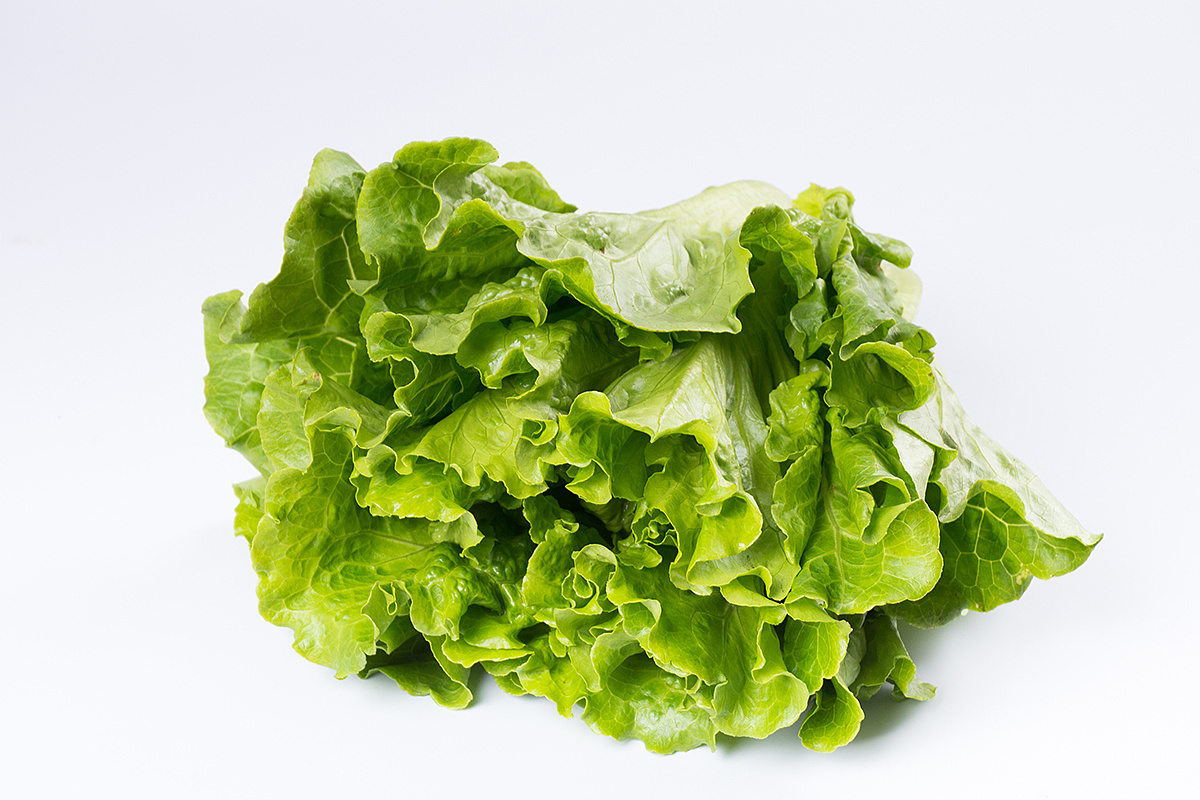
\includegraphics[scale=0.18]{{figure/生菜.jpg}}%插入图片的指令
    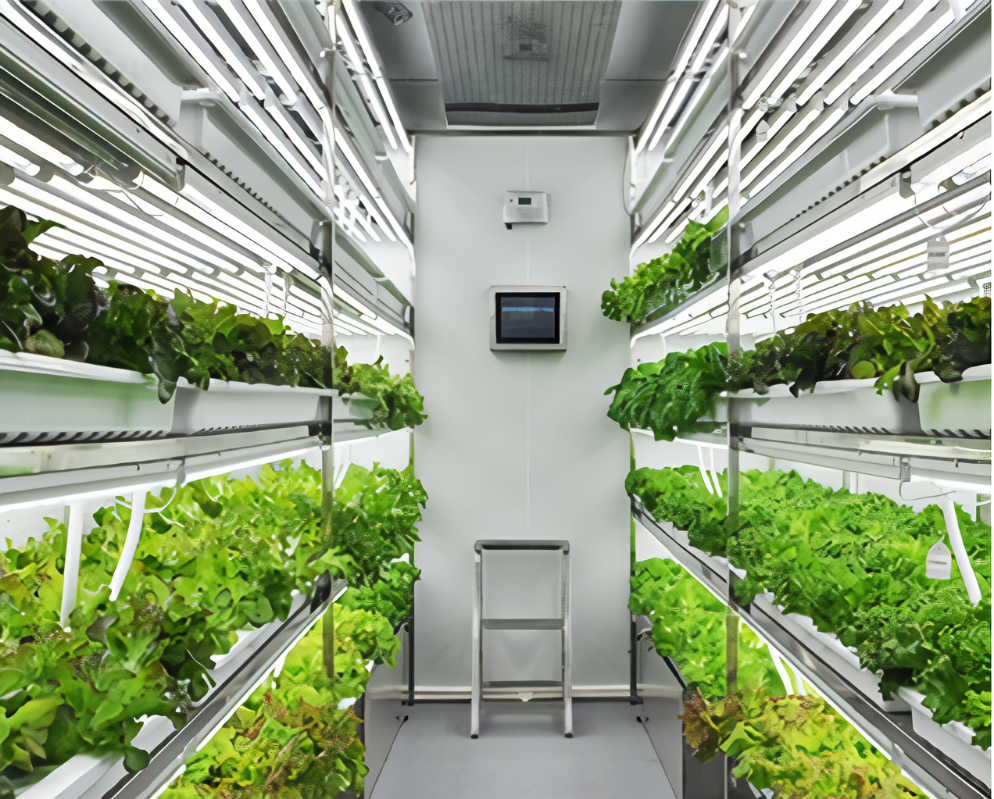
\includegraphics[scale=0.18]{figure/集装箱.png}
    \caption{Lettuce(Left) and Interior of a Container Plant Factory(Right)}%标题
    \label{Label}
\end{figure}

However, maintaining a suitable growing environment for lettuce requires a lot of energy, which can result in high energy costs if the container plant is not optimized; on the other hand, if the suitable environment is abandoned for energy saving, it will have an impact on the yield and quality of lettuce, and even on sales and thus on income. Therefore, it is necessary to analyze the growth pattern of lettuce and to build a suitable container system accordingly in order to balance the two and reduce the energy consumption per fresh lettuce weight while increasing the crop yield.

\subsection{Restatement of the Problem}



Considering the background information and restricted conditions identified in the problem statement, we need to establish a model that is universal in its applicability to different athletes
and complete the following tasks using the model:    
\begin{itemize}
    \item \textbf{Task 1} asked us to provide a growth model for lettuce that describes the fresh weight of a single lettuce plant as a function of light intensity and temperature. 
    \item In \textbf{Task 2}, we need to give the annual fresh weight of lettuce harvest that can describe a 20-foot container based on the assumed conditions considering planting density and harvesting strategy.
    \item In \textbf{Task 3}, we need to develop a model for calculating the annual air conditioning consumption of a container factory. Besides, We also need a model for calculating the lighting energy consumption of a container factories plant as a 
    function of the intensity of the artificial lighting and planting density.
    \item \textbf{Task 4} required us to develop a model to predict energy consumption per fresh weight of lettuce based on the above model. Also, this task requires us to provide an optimal involved and operational strategy to balance yield and energy consumption.
    \item \textbf{Task 5}  considered temperature regulation through mechanical ventilation. We were required to develop a model to determine the operating strategy of mechanical ventilation and to evaluate its energy-saving potential.
    \item \textbf{Finally}, we need to prepare a one-page article of our findings to MCM Corporation outlining our research.

\end{itemize}
% 任务一要求我们提供一个生菜的生长模型,用于描述单株生菜的鲜重作为光照强度和温度的函数。
% 在集装箱中的空间是有限的,植物也有自己的生长周期。因此在任务二中,我们需要在假设的条件下考虑种植密度和收获策略的基础上给出能够描述20英尺集装箱的生菜收获年鲜重。

% 任务四要求我们根据上述模型,建立一个预测生菜每鲜重耗能的模型,以描述单位产量的能耗如何受到集装箱系统涉及的因数的影响(如种植密度、照明强度、温度等等)。同时该任务还要求我们提供一个最佳的涉及和操作策略,以平衡产量和能源消耗。
% 任务五考虑通过机械通风来调节温度。由于机械通风能耗远低于空调能耗,需要我们开发一个模型确定机械通风的运行策略,并且评估其节能潜力。

\subsection{Our Work}



\begin{figure}[h]
    \centering
    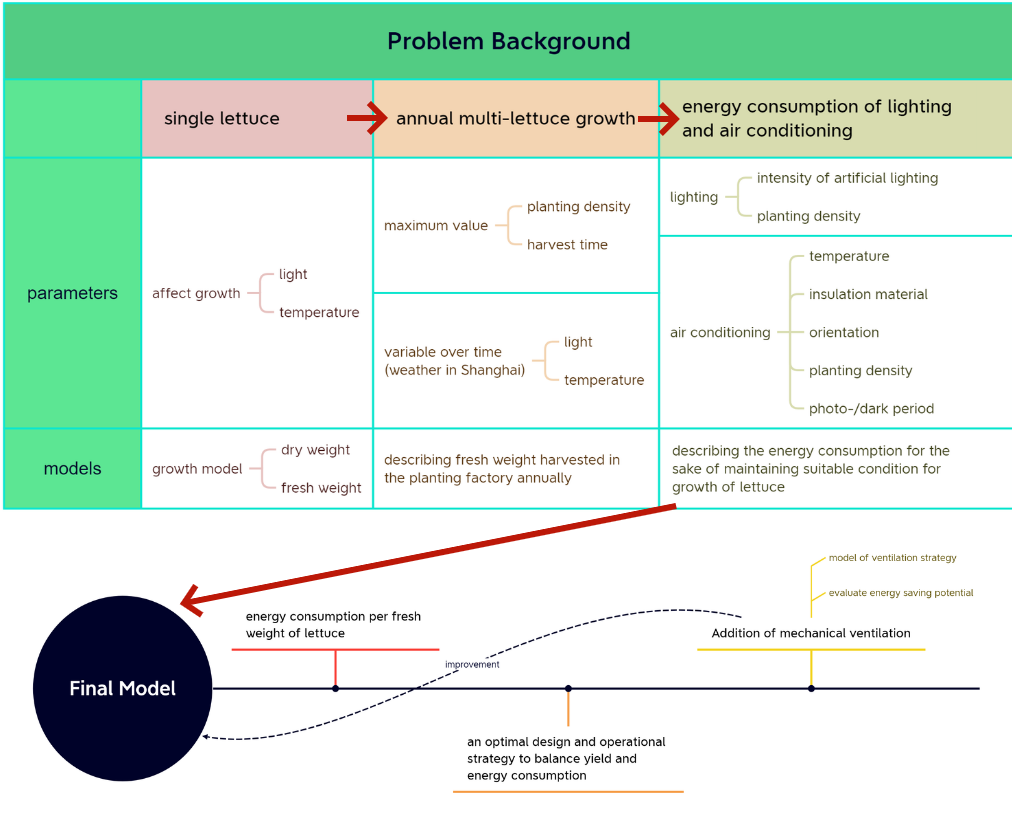
\includegraphics[scale=0.43]{{figure/1.3 OurWork.png}}%插入图片的指令
    \caption{Our Work Structure Graph}%标题
    \label{Label}
\end{figure}

\begin{comment}
我们对任务的背景进行了分析,并建立了模型进行生长预测。我们首先建立了基于单个生菜的生长干重模型。我们对光照和温度两大主要因素进行估计分析,建立了单个生菜的生长模型。我们基于这个单体生长模型,延伸出了有限空间内的年生长鲜重模型。我们思考了种植密度和收获策略,得到了可以在有限集装箱中收获最多生菜鲜重的模型。随后我们加入了集装箱生产的耗能分析,建立了植物工厂完整的生菜生产模型。在这个模型中,我们考虑了照明强度,温度,照明时间等等,并按照生产热量作为分析依据,模拟出了植物工厂的能源消耗。并以机械通风为样本,分析了机械通风的运行策略,并且评估其节能潜力。
\end{comment}

We analyzed the background of the task and built a model for growth prediction. We first developed a growth dry weight model based on individual lettuce. We estimated and analyzed the two main factors, light and temperature, to build a growth model for a single lettuce. We extended the annual growth fresh weight model in a limited space based on this single growth model. We thought about the planting density and harvesting strategy to obtain the model that can harvest the maximum fresh weight of lettuce in a finite container. We then added the energy consumption analysis of container production to build a complete lettuce production model for plant factories. In this model, we considered lighting intensity, temperature, lighting time, etc., and simulated the energy consumption of the plant factory according to the heat production as the basis of analysis. We also analyzed the operation strategy of mechanical ventilation as a sample and evaluated its energy saving potential.

